\documentclass[a4paper,10pt]{article}

\usepackage[latin1]{inputenc}
\usepackage{graphicx}
\usepackage{url}
\usepackage{palatino}
%%\usepackage{rotating}

\begin{document}

\title{ATiSA Exercise 1: Software Architecture Description of the HS07 System}

\author{
  $$Gerado Adelizzi,\\
   Ivan Valencik, \\
   Daniel Ashaiik Mac Donald,\\ 
   Martin Norre Christensen$$\\\\
  Department of Computer Science, University of Aarhus\\
  Aabogade 34, 8200 {\AA}rhus N, Denmark\\\\
  \makeatletter
  Reenskaug\\\\
  20108627\\ 20108624\\ 20022432\\ 20084414\\\\
  gerado@cs.au.dk\\ valencik@gmail.com\\ danielneroshadow@gmail.com\\ mnc@cs.au.dk
}

\date{01-02-11}

\maketitle

% =====================================================================
\begin{abstract}
  The HS07 system implements a closed-loop control of the heating in a
  private home. It monitors thermometers in the home, and based on
  measurements HS07 adjusts radiators in the home. This report gives a
  software architecture description of an architectural prototype of
  the HS07 system. The techniques used for architectural description
  are taken from \cite{christensen2004archdesc}.
\end{abstract}

% =====================================================================
\section{Introduction}

Figure~\ref{fig:hs07} shows a schematic overview of HS07 in a
home. The home may be accessed by the home owner from the outside
through the HS07 gateway. The HS07 gateway also monitors and controls
the home.

\begin{figure}[!htb]
	\centering
		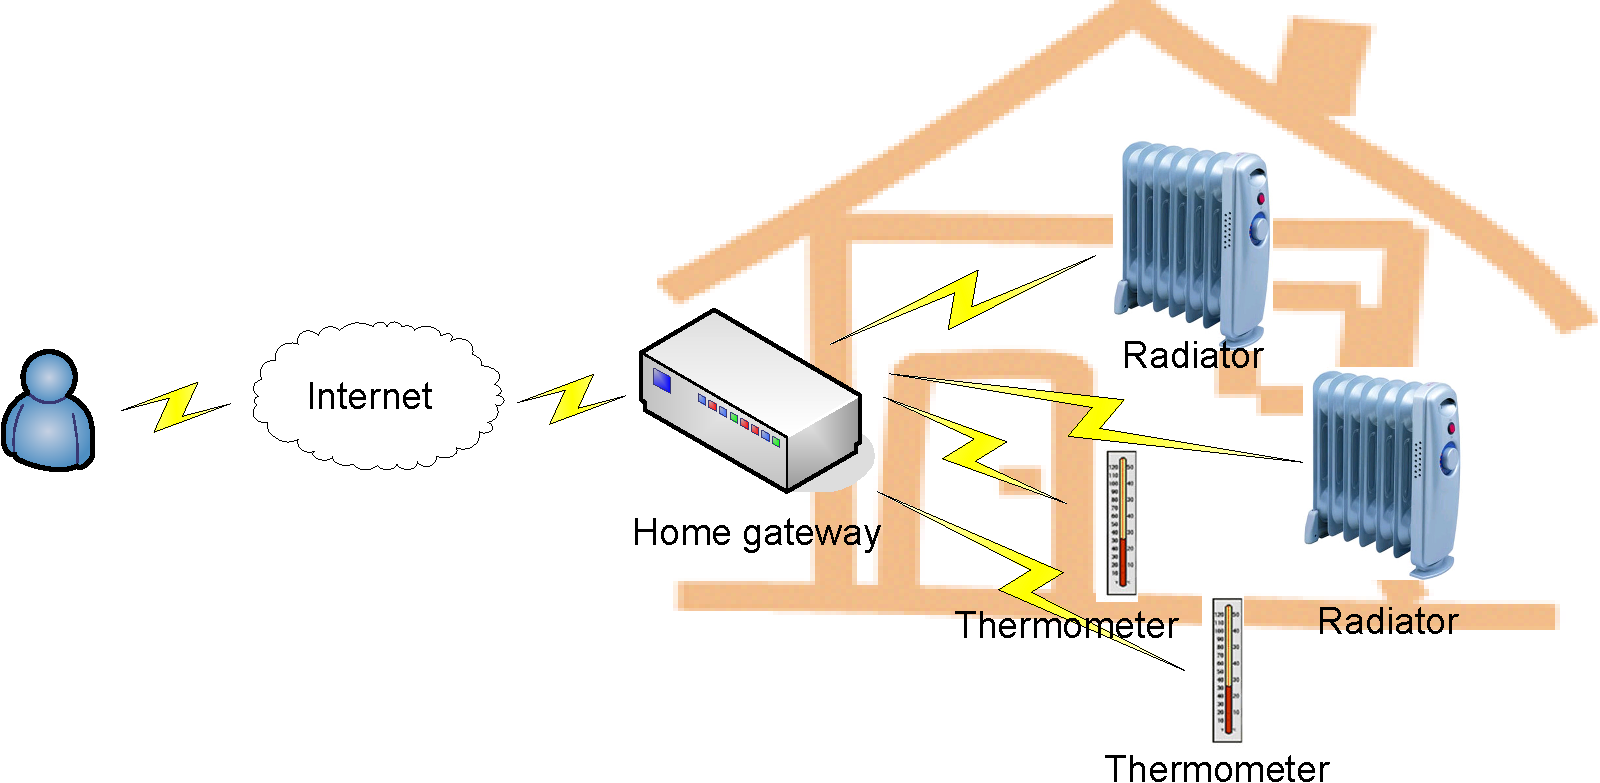
\includegraphics[scale=0.4]{figures/hs07.pdf}
		\caption{HS07 in a home}
		\label{fig:hs07}
\end{figure}


HS07 includes sensor and actuator hardware which runs on an embedded Java virtual
machine with standard software.

% =====================================================================
\section{Architectural Requirements}

For our purposes there is one main use case for the HS07 system:
\begin{quote}
  \emph{Control Temperature}: The gateway collects measurements from
  thermometers and reports this to radiators that then control the
  temperature.
\end{quote}

The major driving qualities attributes of the HS07 system
are\footnote{These qualities will be operationalized in Exercise 2}:

\begin{itemize}
\item \emph{Performance.} HS07 should be performant so that a large
  number of thermometers and radiators may be part of the system.
\item \emph{Modifiability.} It must be possible to modify HS07 to
  include new types of sensors and actuators.
  \item \emph{Availability.} The system may not be unavailable for too long. Otherwise if the radiators keep
being turned on while temperatures rise, that could be fatal.
\end{itemize}


% =====================================================================
\section{Architectural Description}


% ---------------------------------------------------------------------
\subsection{Module Viewpoint}
\begin{center}
	\centering
		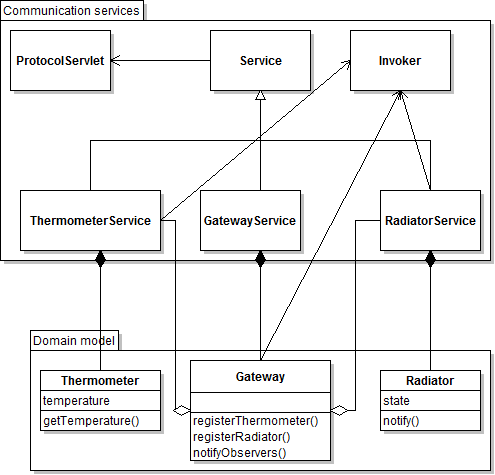
\includegraphics[scale=0.4]{figures/moduleview.png}
	\label{fig:moduleview}
\end{center}
% ---------------------------------------------------------------------
\subsection{Component \& Connector Viewpoint}
\begin{center}
	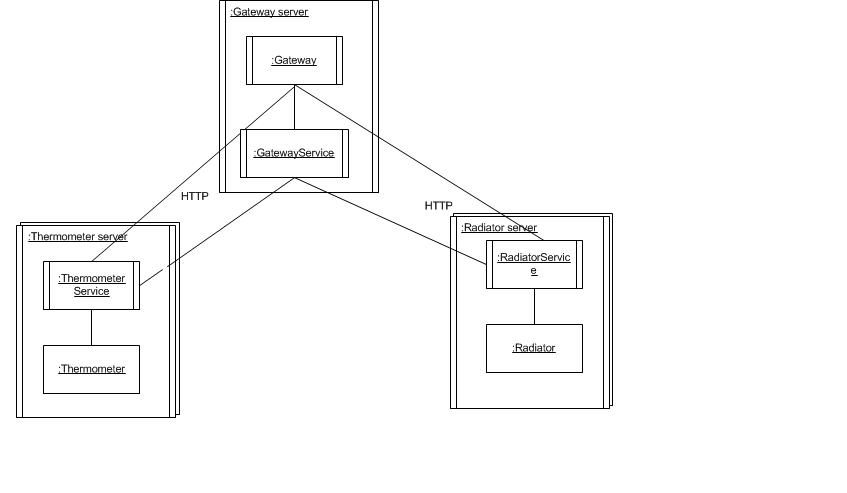
\includegraphics[scale=0.6]{C:/Users/martin/Desktop/hs07-latex/report-template/figures/c&c1.jpg}
\end{center}
\subsubsection{Responsibilities}
\begin{itemize}
	\item \emph{Gateway}\\Gets current temperature from thermometers\\Informs radiators about current temperature
	\item \emph{GatweayService}\\Make the gatway accesible over a network
	\item \emph{Thermometer}\\Measures temperature
	\item \emph{Thermometer service}\\Make the thermometer accesible over a network
	\item \emph{Radiator}\\Turns heating on and off depending on a given temperature
	\item \emph{Radiator service}\\Make the thermometer accesible over a network
\end{itemize}
% ---------------------------------------------------------------------
\subsection{Allocation Viewpoint}
\begin{center}
	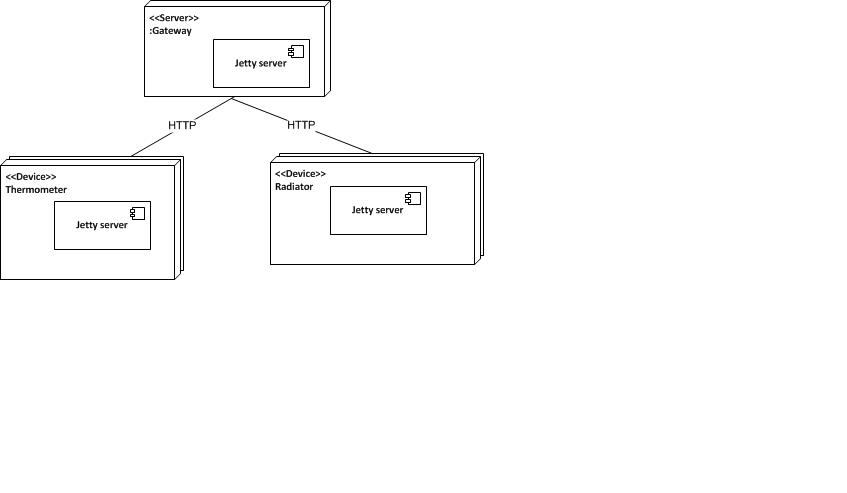
\includegraphics[scale=0.6]{C:/Users/martin/Desktop/hs07-latex/report-template/figures/allocationview.jpg}
\end{center}
\begin{itemize}
	\item Environmental
\begin{itemize}
	\item Gateway is a device that communicates with the outside world, and also monitors and controls the home.
	\item Thermometer is a device that measures the temperature and communicates the temperature to the gateway.
	\item Radiator is a device that makes a decision about whether making heat or not depending on the temperature it gets from the gateway.
\end{itemize}
	\item Software elements\\
Each device contains a Jetty server that they use for the communication. A Jetty server is a java web server and depending on the device it runs the following software components:
	
\begin{itemize}
	\item Gateway: One GatewayServer
	\item Thermometer: One ThermometerServer
	\item Radiator: One RadiatorServer
\end{itemize}
\end{itemize}

% =====================================================================
\section{Discussion}
\subsection{Strengths}
A strength of this approach is that it does describe more than just class diagrams and sequence diagrams would do.
\subsection{Limitations}
A limitation of this approach is that the people who uses the architecture need to know about it and understand it well before being able to use it good. This could cause misunderstanding in the communication of the architecture. Another limitation is that it probably won't do good for programming lanugages that are not object-oriented. Furhermore in the allocation view it is hard to express that one component is shared between nodes. E.g. when a library is present at more than one node, the only way to express it is to put the component into every node.

\subsection{Are there aspects of the software architecture that have not been
properly described?}
Except for the limitation that the allocation view cannot show that a component is shared, we think it pretty much describes everything for now.

% =====================================================================
\section{Further discussion}
\subsection{For the architectural description above, discuss what (if anything) should be changed or added for it to comply with the IEEE recommended practice for architectural description}
Compared to the IEEE recommended practice there are many things that we haven't done. E.g. the recommended practice asks for the points copied in below.\\\\
a) AD identifcation, version, and overview information \\
b) Identifcation of the system stakeholders and their concerns judged to be relevant to the architecture\\
c) Specifcations of each viewpoint that has been selected to organize the representation of the architecture and the rationale for those selections
d) One or more architectural views \\
e) A record of all known inconsistencies among the architectural description�s required constituents\\
\\
f) A rationale for selection of the architecture\\\\

The point d) we have definitely done. For c) we have made some specification about responsibilitys in the C&C view, but we probably don't have enough detail to live up to the point. The other points we believe we can say that we haven't done.

\subsection{Consider the definition of software architecture by [Perry and Wolf, 1992]. Discuss what the 'elements', 'form', and 'rationale' according to this definition would be for the HS07 system}
\subsubsection{Elements}
In our case the connecting elements are the classes which makes the communication possible, which are the gateway plus all those from the communication package in the module view. The processing elements are the gateway (it calculates the average temperature) and the radiators. The data elements are the thermometer.
\subsubsection{Form}
Properties are the properties that we have put in the architectual views. E.g. on the allocation view we have stated that the system should be using a Jetty server. That is a property, which does that the implementator then cannot decide to use an alternative without conflicting with the architecutre. The relationsships basically are the edges and the packages that we have drawn in our diagrams.
\subsubsection{Rationale}
Rationale is about arguing why a given architecture is chosen. Our architectual description doesn't really have a rationale, since we have been given the code.
% =====================================================================
\bibliography{paper}
\bibliographystyle{apalike}


\end{document}


